\documentclass[a4paper, 12pt]{article}

\usepackage[T2A]{fontenc}
\usepackage[utf8]{inputenc}
\usepackage[english,russian]{babel}
\usepackage[left=15mm, top=20mm, right=15mm, bottom=20mm, nohead, nofoot]{geometry}

\usepackage{hyperref}
\usepackage{graphicx}
\usepackage{wrapfig}
\usepackage{afterpage}
\usepackage{amsmath, amsfonts, amssymb, amsthm, mathtools}
\author{Хомутов Андрей, группа Б06-903}
\title{ВПВ по курсу "Электричество и магнетизм" \\ Конденсатор на высоких частотах}
\date{22 декабря 2020 г.}
%%%%%%%%%%%%%%%%%%%%%%%%%%%%%%%%%%%%%%%%%%%%%%%%%%%%%%%%%%%%%%%%%%%%%%%%%
\usepackage{graphicx, wrapfig, subcaption, setspace, booktabs}
\usepackage[protrusion=true, expansion=true]{microtype}
\usepackage[english]{babel}
\usepackage{sectsty}
\usepackage{url, lipsum}
\newcommand{\HRule}[1]{\rule{\linewidth}{#1}}
\onehalfspacing
\setcounter{tocdepth}{5}
\setcounter{secnumdepth}{5}
%%%%%%%%%%%%%%%%%%%%%%%%%%%%%%%%%%%%%%%%%%%%%%%%%%%%%%%%%%%%%%%%%%%%%%%%%


\begin{document}

\title{ \normalsize \textsc{Лабораторная работа по физической химии}
		\\ [4.0cm]
		\HRule{0.5pt} \\ [0.3cm]
		\LARGE \textbf{{Активность и коэффициент активности ионов 
		в растворах, pH-метрия}}
		\HRule{0.5pt} \\ [0.1cm]
		\normalsize  \vspace*{18\baselineskip}}

\date{}

\author{Шамарина Екатерина, Б06-903 \\
		Хомутов Андрей, Б06-903 \\
ФБМФ, 2020\\ }

\maketitle
\thispagestyle{empty}
\newpage

\section*{Цели работы} 
\begin{enumerate}
    \item Знакомство с потенциометрическими методами определения среднеионных коэффициентов активности электролитов и измерения pH растворов; 
    \item исследование зависимости среднеионного коэффициента активности электролита от его концентрации; 
    \item приобретение практических навыков измерения pH.
\end{enumerate}

 
\section{Теоретическая часть}
\subsection{Химический потенциал и активности компонентов раствора}
Химический потенциал компонента идеального раствора:
\begin{equation}
\mu_{i}(T, p, x)=\mu_{i}^{0}(T, p)+R T \cdot \ln x_{i}
\end{equation}
где $\mu_{i}^{0}=\mu_{i}\left(T, p^{0}, x_{i}=1\right)$ – стандартный потенциал i- го компонента при равенстве мольной доле равной единице, заданной температуре T и давлении в один бар. Химический потенциал компонента реального раствора вводится аналогично:
\begin{equation}
\mu_{i}(T, p, x)=\mu_{i}^{0}(T, p)+R T \cdot \ln a_{i}
\end{equation}
где $\mu_{i}^{0}=\mu_{i}\left(T, p^{0}, a_{i}=1\right)$ – стандартный потенциал i-го компонента.
Активность – безразмерная величина, которая непосредственно выражается через химический потенциал. Она не связана напрямую с его мольной долей, хотя и зависит от нее. Это термодинамическая величина, выражающая вклад компонента в свободную энергию Гиббса раствора:
\begin{equation}
G(T, p, x)=\sum \nu_{i} \mu_{i}=\sum \nu_{i} \cdot\left(\mu_{i}^{0}+R T \cdot \ln a_{i}\right)
\end{equation}

\subsection{Теория Дебая-Хюккеля}
Теория Дебая-Хюккеля позволяет представить коэффициент активности i-го иона в виде разницы энергии иона типа i в реальном растворе ионной силы I и в предельном случае,когда ионы вокруг него отсутствуют, I= 0:
\begin{equation}
R T \cdot \ln \gamma_{i}=N_{a} \cdot \Delta U=N_{a} \cdot\left(U_{I}-U_{I=0}\right)
\end{equation}
Для расчета энергии производится интегрирование уравнения Пуассона-Больцмана и в предельном случае $ez_{i} \varphi(r) \ll k T$ получают следующий результат(первое приблежение Д-Х) для водных растворов при температуре 25°C:
$$
\lg \gamma_{i} \approx-0.51 z_{i}^{2} \sqrt{I}
$$
Измерить активность ионов одного типа не удается, так как нельзя создать систему с ионами только одного типа - она не будет электронейтральной. Измерению
поддаются только активности ионов при наличии ионов, компенсирующих их заряд.
Для такой системы принято говорить о среднеионном коэффициенте активности, который вводится перераспределением соответствующих вкладов в свободную
энергию поровну между ионами каждого сорта. Так для электролита, диссоцииру-
ющего в растворе по схеме: 
$$
\mathrm{M}_{\nu_{+}} \mathrm{A}_{\nu_{-}} \rightleftarrows \nu_{+} \mathrm{M}^{z+}+\nu_{-} \mathrm{A}^{z-}
$$
среднеионный коэфф. активности выражается как:
\begin{equation}
\gamma_{\pm}^{\nu}=\gamma_{+}^{\nu_{+}} \gamma_{-}^{\nu_{-}}
\end{equation}
Среднеионный коэффициент активности в первом приближении теории Дебая–Хюккеля для концентраций в моль/л при 25°C (справедливо при I < 0.01M):
\begin{equation}
\lg \gamma_{\pm} \approx-0,51\left|z_{+} z_{-}\right| \sqrt{I}
\end{equation}
Во втором приближении при I <0,1M учитывается то, что центры ионов не могут сблизится на расстояние, меньше некоторого a. Во многих случаях работает формула Гютельберга для водных растворов при 25°C, соответствующая a≈0,48nm:
\begin{equation}
\lg \gamma_{\pm}=-0.51\left|z_{+} z_{-}\right| \frac{\sqrt{I}}{1+\sqrt{I}}
\end{equation}
В качестве третьего приближения для широкого диапазона изменения концентраций используют полуэмпирическую формулу со свободным членом b (константа высаливания):
\begin{equation}
\lg \gamma_{\pm}=-0,51\left|z_{+} z_{-}\right| \frac{\sqrt{I}}{1+\sqrt{I}}+b I
\end{equation}
\subsection{О потенциометрическом измерении pH}
Величина водородного потенциала pH определяется активностью ионов водорода в растворе:
\begin{equation}
p H=-\lg a_{H^{+}}
\end{equation}
Под электродом понимают систему, состоющую из нескольких фаз, на границе которых направленное движение электронов (носителей заряда) меняется на направленное движение ионов или наоборот. Как правило, для измерения pH используют два электрода:индикаторный(потенциал которого меняется в зависимости от pH исследуемого раствора) электрод сравнения.
\subsubsection{Хлорсеребряный электрод}
Представляет собой серебряную проволочку, покрытую слоем труднорастворимой соли AgCl в растворе электролита, содержащего хлорид-ионы Cl− (обычно это насыщенный или 3.5 М раствор KCl). Полуреакция для хлорсеребряного электрода может быть записана так:
$$
\mathrm{AgCl}_{(s)}+e^{-} \rightleftarrows \mathrm{Ag}_{(s)}^{0}+\mathrm{Cl}_{(s o l)}^{-}
$$
Используя уравнение Нернста и ПР AgCl, можно показать, что потенциал такого электрода определяется активностью хлорид-ионов (в растворе KCl):
\begin{equation}
\varphi=\varphi^{0}+\frac{R T}{F} \ln a_{\mathrm{Ag}^{+}}=\varphi^{0}+\frac{R T}{F} \ln \Pi \mathrm{P}_{\mathrm{AgCl}}-\frac{R T}{F} \ln a_{\mathrm{Cl}^{-}}=\varphi_{2}^{0}-\frac{R T}{F} \ln a_{\mathrm{Cl}^{-}}
\end{equation}
В электрохимических ячейках такой электрод часто используется в качестве
электрода сравнения, поскольку он обладает постоянным и хорошо воспроизводимым потенциалом (который задается концентрацией электролита KCl, в который
помещена Ag проволочка). 
\subsubsection{Стеклянный электрод}
Представляет собой трубку с мембраной в виде шарика из специального стекла, выдуваемого на конце трубки. Внутрь шарика заливают стандартный раствор с известным значением pH (зачастую это 0,1 М раствор HCl). Уравнение, описывающее потенциал стеклянного электрода, было получено Б.П. Никольским:
\begin{equation}
\varphi=\varphi_{1}^{0}+\frac{R T}{F} \ln \left(a_{\mathrm{H}^{+}}+K a_{\mathrm{Na}^{+}}\right)
\end{equation}
Если вклад от активности ионов H+ преобладает над вкладом ионов Na+, что выполняется в кислых и нейтральных средах, то
\begin{equation}
\varphi \approx \varphi_{1}^{0}+\frac{R T}{F} \ln a_{\mathrm{H}^{+}}
\end{equation}
При большой концентрации катионов Na+ (а также в меньшей степени Li+, K+ и др.), в сравнительно щелочной среде, возникают значительные отклонения водородной функции электрода E(pH) от линейной зависимости. Это называют щелочной
(или катионной) ошибкой стеклянного электрода.



\newpage
\section{Практическая часть}
\subsection{Калибровка pH-метра}
По набору стандартных буферных растворов, а именно растворов с рН: 1,68, 4, 7, 10, была построена калибровочная прямая ЭДС от рН стандартного буферного раствора для комбинированного электрода.
\begin{table}[h]
\begin{center}
\caption{ЭДС(рН) для комбинированного электрода}
\begin{tabular}{|c|c|c|c|c|}
\hline
pH      & 10  & 7    & 4     & 1.68  \\ \hline
ЭДС, мВ & -63,8     & 93,9 & 264,3 & 392,8 \\ \hline
\end{tabular}
\end{center}
\end{table}

Как видно, наклон графика составляет 55.1 мВ (рис. 1), что практически соответствует 59.1 мВ $=\frac{R T}{F} \ln 10$ из теории.

\begin{figure}[h!]
    \begin{center}
    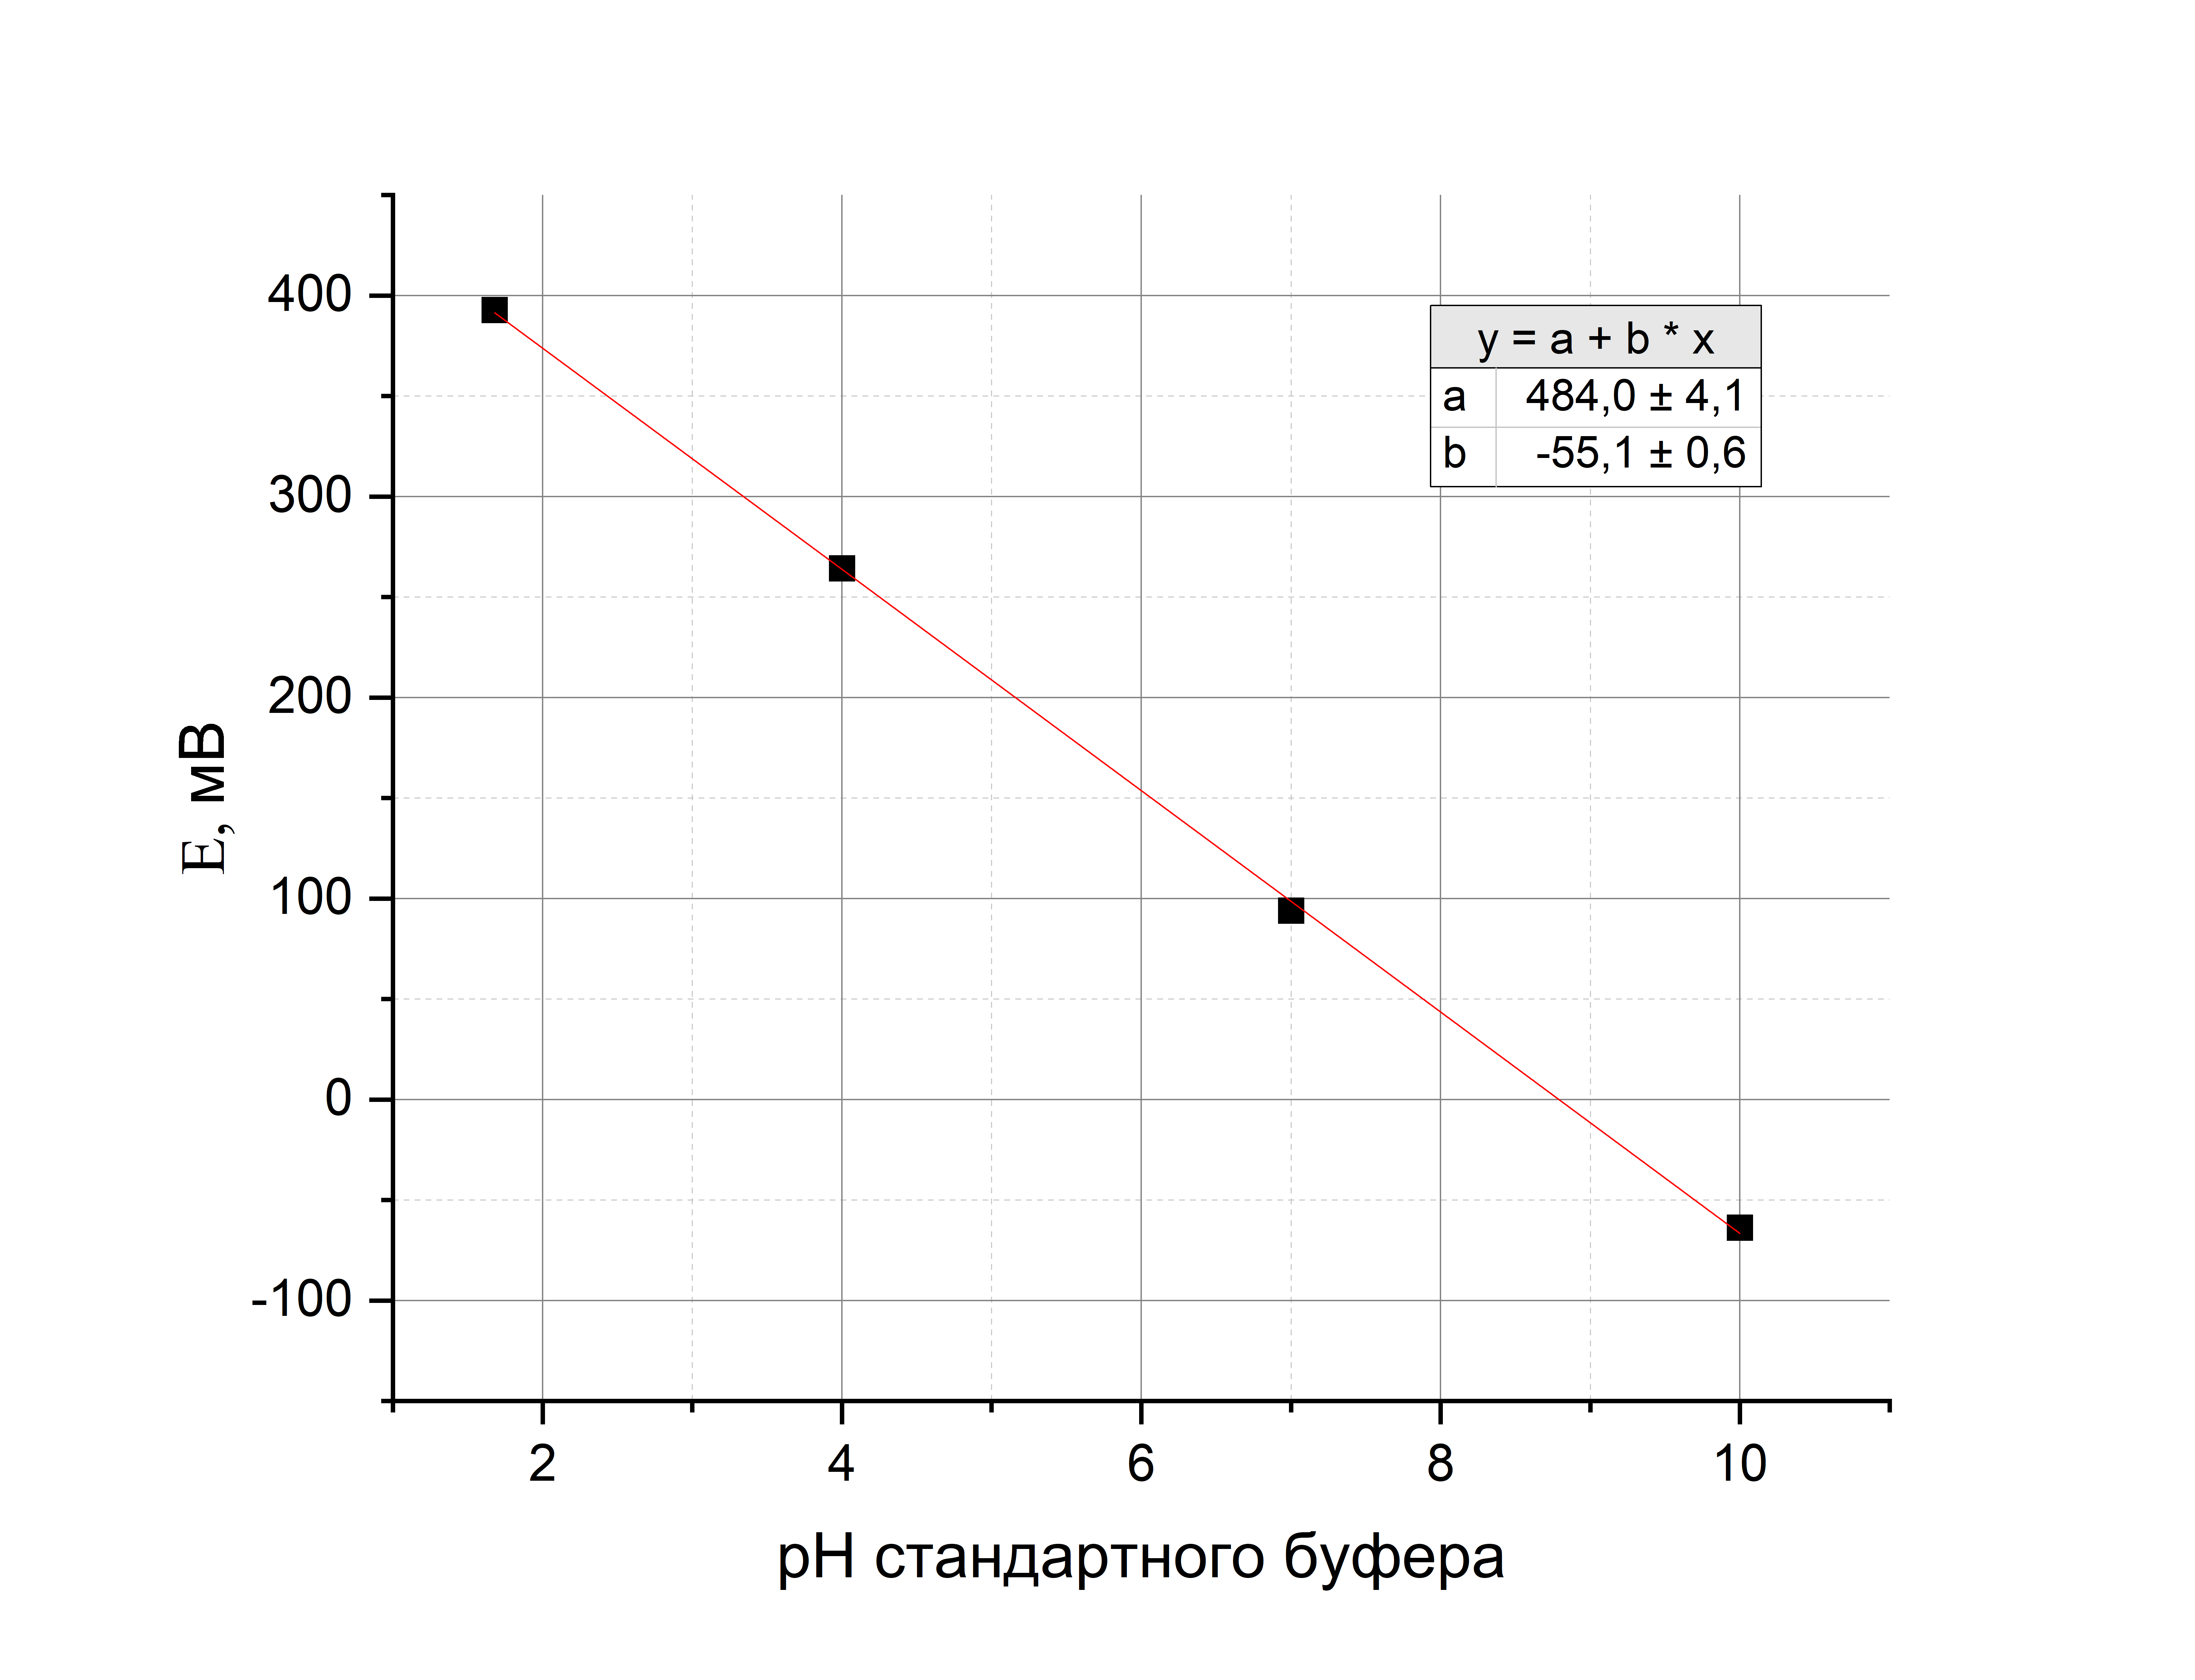
\includegraphics[width=0.8\textwidth]{1.1.png}
    \end{center}
    \caption{ЭДС комбинированного электрода в зависимости от pH}
\end{figure}


%\subsubsection{Определение магнитного момента,намагниченности и остаточной магнитной индукции вещества магнитных шариков}

\subsection{Определение активности $H^{+}$ и среднеионного коэффициента активности}
\subsubsection{Измерение ЭДС при добавлении HCl}
Сначала строится зависимость ЭДС на комбинированном и некомбинированном электродах при постепенном добавлении двухмолярной соляной кислоты к дистиллированной воде (см. таблицу 2). 

\begin{table}[h!]
\begin{center}
\caption{Измерение ЭДС при добавлении HCl}
\begin{tabular}{|c|c|c|c|c|c|}
\hline
\begin{tabular}[c]{@{}c@{}}Добавленный\\ объем HCl, мл\end{tabular} & \begin{tabular}[c]{@{}c@{}}Общий объем\\ HCl в р-ре, мл\end{tabular} & С(HCL), моль/л & -lg(C)  & \begin{tabular}[c]{@{}c@{}}ЭДС НЕомбин.,\\ мВ\end{tabular} & \begin{tabular}[c]{@{}c@{}}ЭДС комбин,\\ мВ\end{tabular} \\ \hline
0,1                                                                 & 0,1                                                                  & 0,004          & 2,39881 & 88,1                                                       & 383                                                      \\ \hline
0,4                                                                 & 0,5                                                                  & 0,020          & 1,70329 & 164,5                                                      & 410                                                      \\ \hline
0,5                                                                 & 1                                                                    & 0,039          & 1,40654 & 197,5                                                      & 418                                                      \\ \hline
1                                                                   & 2                                                                    & 0,077          & 1,11394 & 230,4                                                      & 426                                                      \\ \hline
1                                                                   & 3                                                                    & 0,113          & 0,94612 & 249,2                                                      & 430,7                                                    \\ \hline
1                                                                   & 4                                                                    & 0,148          & 0,82930 & 262,5                                                      & 435,2                                                    \\ \hline
1                                                                   & 5                                                                    & 0,182          & 0,74036 & 272,9                                                      & 439,5                                                    \\ \hline
5                                                                   & 10                                                                   & 0,333          & 0,47712 & 302,2                                                      & 449,6                                                    \\ \hline
10                                                                  & 20                                                                   & 0,571          & 0,24304 & 331,2                                                      & 459,6                                                    \\ \hline
10                                                                  & 30                                                                   & 0,750          & 0,12494 & 347,2                                                      & 465,6                                                    \\ \hline
10                                                                  & 40                                                                   & 0,889          & 0,05115 & 357,6                                                      & 471,7                                                    \\ \hline
10                                                                  & 50                                                                   & 1,000          & 0,00000 & 365,4                                                      & 475,5                                                    \\ \hline
\end{tabular}
\end{center}
\end{table}

По результатам измерений строятся линейные аппроксимации зависимостей ЭДС от $p C_{\mathrm{H}}=-\lg C_{\mathrm{HCl}}$ для обоих электродов (рис. 2). По формулам углы наклона (от рН) должны отличаться в два раза и составить -59.1 мВ и -118.3 мВ для комбинированного и некомб. соответсвенно. Получили (-35.9+-1.7)мВ для комб. и (-115.2+-1.2) для некомб. Это может быть объяснено тем, что измерения на некомб эл-де было возможно провести с точностью 0.1мВ, в то время как показания комбинированного не устанавливались даже в пределах 4мВ. 

\begin{figure}
    \begin{center}
    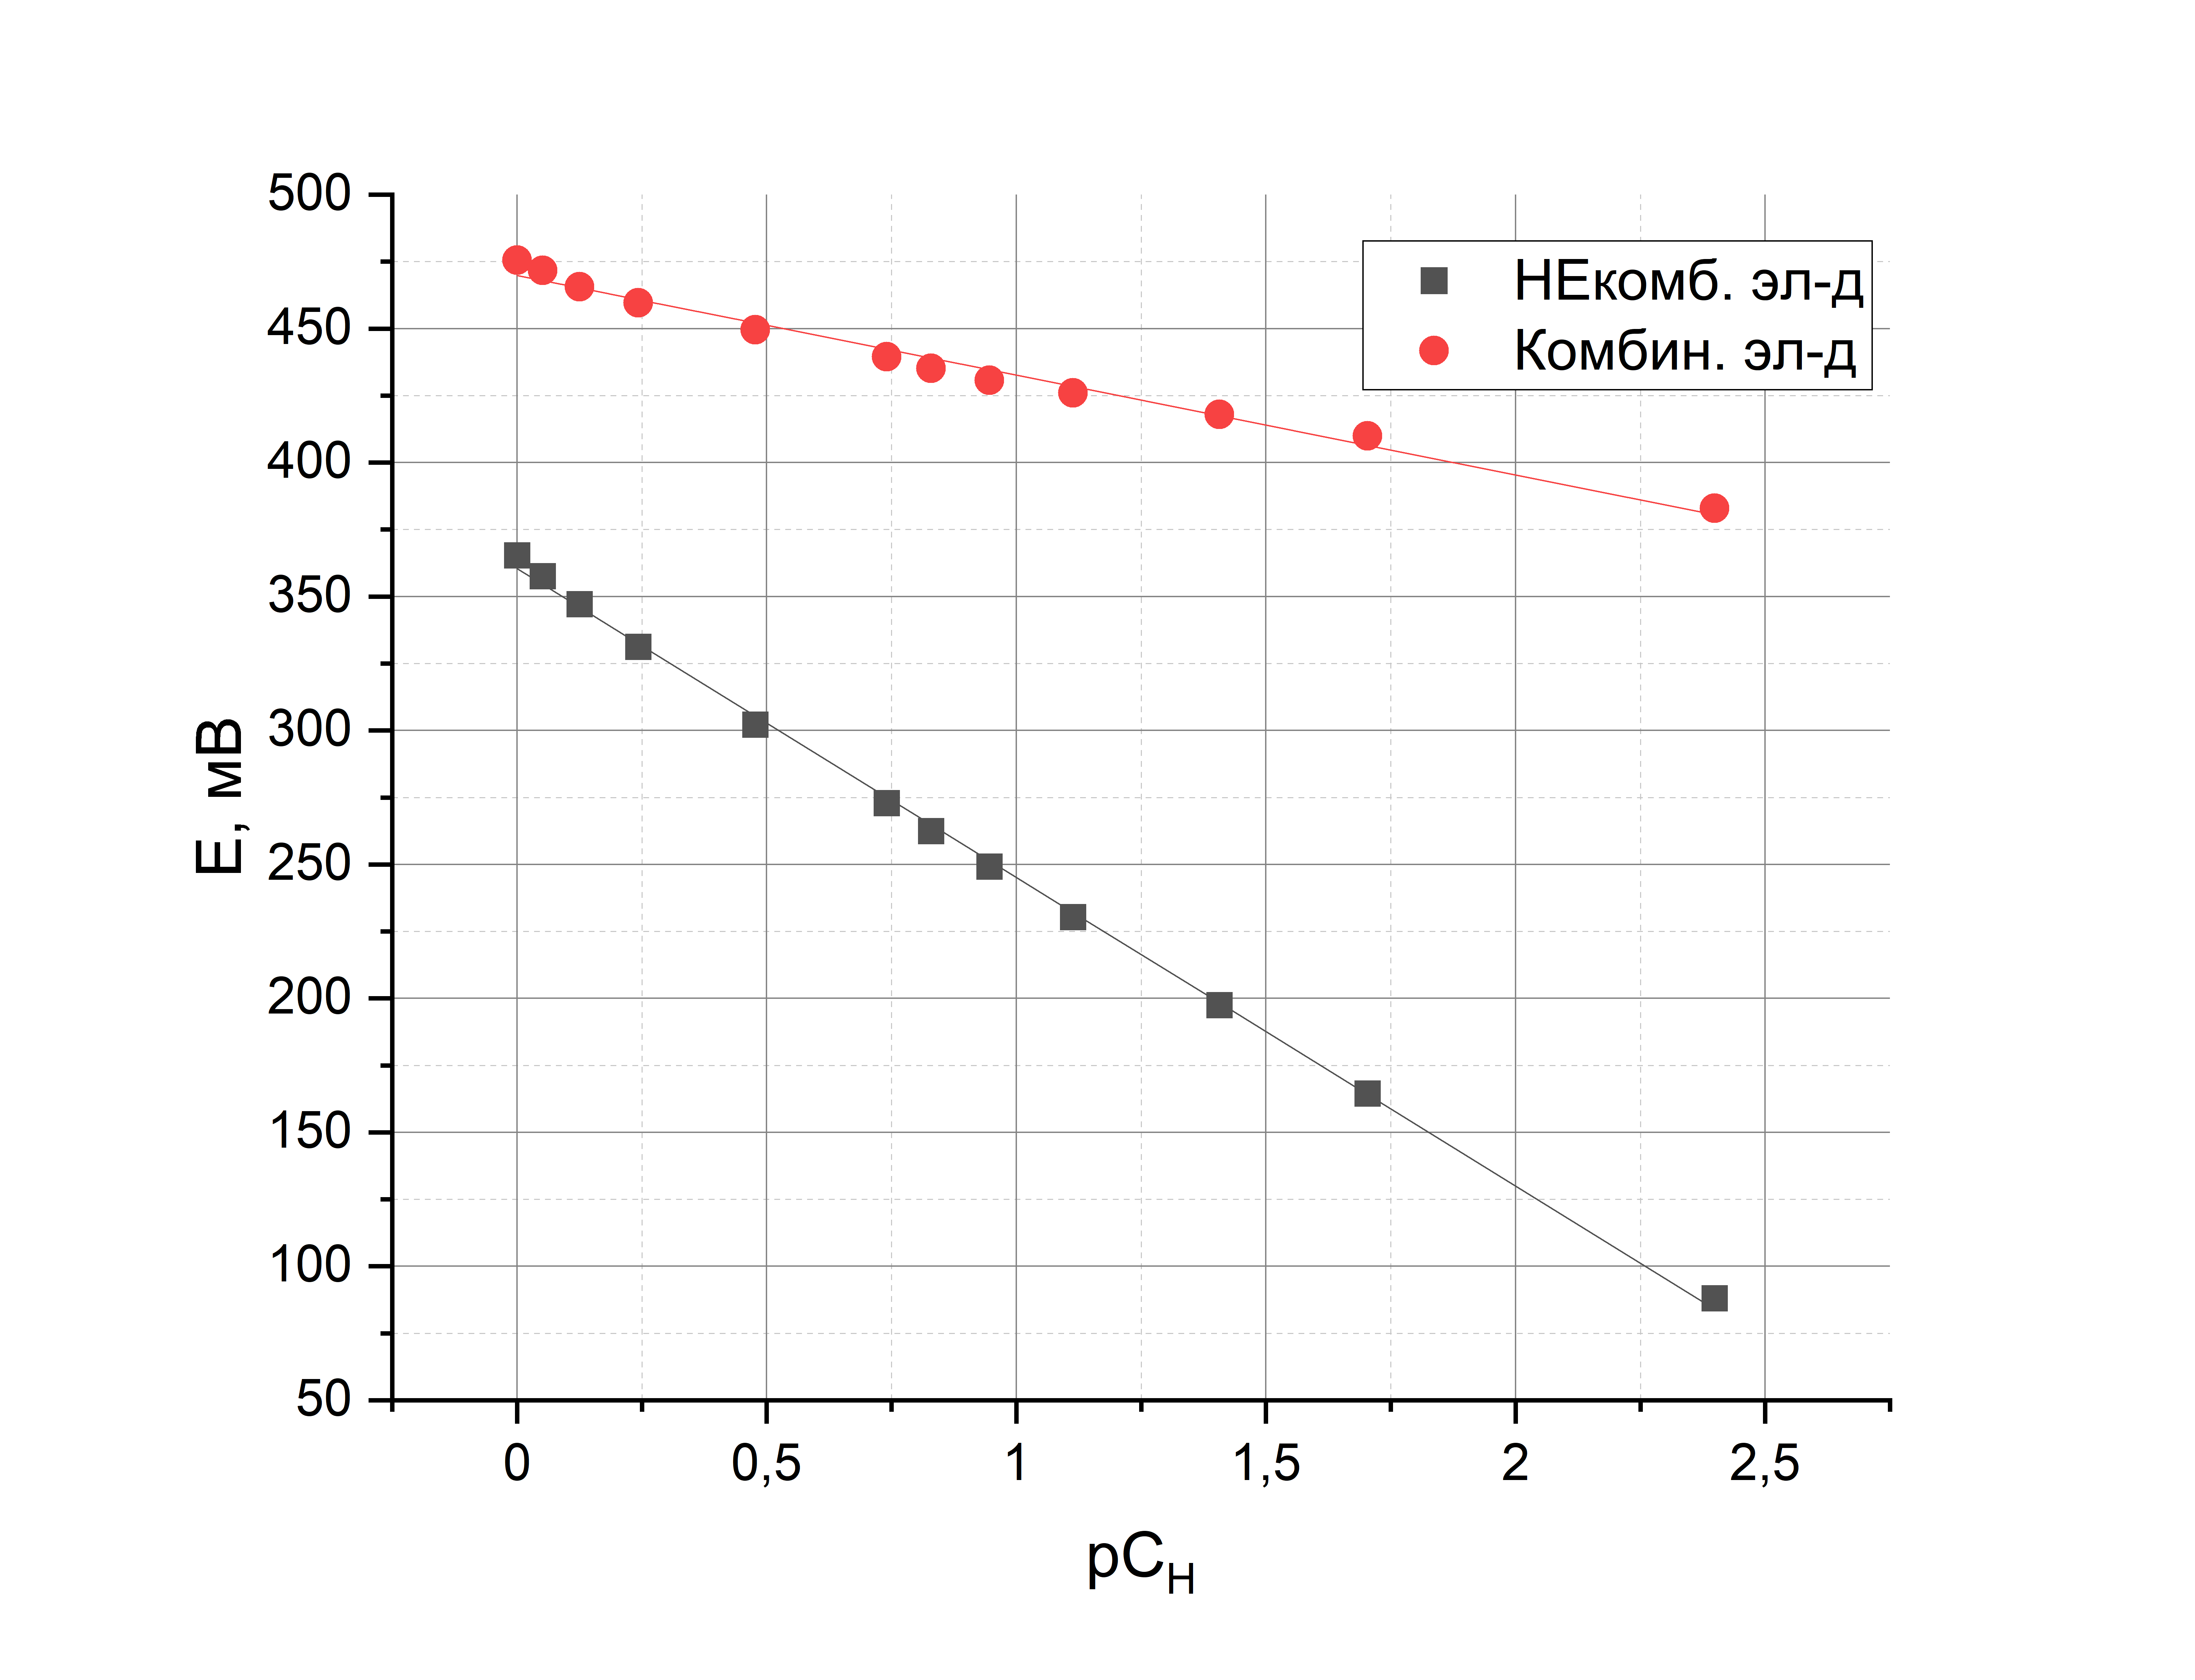
\includegraphics[width=0.7\textwidth]{2.1.png}
    \end{center}
    \caption{ЭДС электродов в зависимости от концентрации HCl}
\end{figure}

\subsubsection{Дальнейший анализ серии измерений для некомб. эл-да}
Зная что для некомб. эл-да:
\begin{equation}
E_{X}=E_{i n d}-E_{r e f}=E^{0}+\frac{R T}{F} \ln a_{H^{+}}^{(X)} a_{\mathrm{Cl}^{-}}^{(X)}=E^{0}+\frac{R T}{F} \ln 10 \cdot \lg \left(\gamma_{\pm} C_{\mathrm{HCl}}\right)^{2}
\end{equation}
\begin{equation}
E_{X}=E^{0}+\frac{2 R T}{F} \ln 10 \cdot \lg \left(\gamma_{\pm} C_{\mathrm{HCl}}\right)
\end{equation}
Воспользуемся результатами теории Дебая-Хюккеля для нашего случая:
\begin{equation}
I=\frac{1}{2} \sum C_{i} z^{2}_{i}=C_{H C l}
\end{equation}
В третьем приближении выражаем среднеионный коэфф. активности как
\begin{equation}
\lg \gamma_{\pm}=-0.51\left|z_{+} z_{-}\right| \frac{\sqrt{I}}{1+\sqrt{I}}+b I \text{, где} b=0.1\left|z_{+} z_{-}\right|=0.1
\end{equation}
И подставляем в уравнение для потенциала
\begin{displaymath}
E_{X}=E^{0}+\frac{2 R T}{F} \ln 10 \cdot (\lg \left(\gamma_{\pm} + \lg C_{\mathrm{HCl}}\right))=  
\end{displaymath}
\begin{displaymath}
=E^{0}+\frac{2 R T \ln 10}{F} \cdot \lg C_{\mathrm{HCl}}+\frac{2 R T \ln 10}{F} \cdot (-\frac{0.51 \sqrt{C_{\mathrm{HC}}}}{1+\sqrt{C_{\mathrm{HCl}}}} +bI)
\end{displaymath}
Далее проанализируем зависимость величины $y$ от концентрации соляной кислоты:
\begin{equation}
y  \equiv E_{X}-\frac{2 R T \ln 10}{F} \cdot \lg C_{\mathrm{HCl}}+\frac{2 R T \ln 10}{F} \cdot \frac{0.51 \sqrt{C_{\mathrm{HC}}}}{1+\sqrt{C_{\mathrm{HC}}}} = E^{0} + \frac{2 R T \ln 10}{F} \cdot bI
\end{equation}
Сама зависимость представлена на рис. 3. Экстраполяцией графика к нулю находим\\ $E^{0} = 373.6 \pm 0.2$мВ. Зная $E^{0}$, c помощью (14) для каждой точки серии измерений б) рассчитаны коэффициенты активности $\gamma_{\pm}$(табл. 3) и построен график зависимости $ lg \gamma_{\pm}$ от корня квадратного из ионной силы раствора (рис.4). Также на графике для наглядности приведены зависимости, вытекающие из первых трех приближений Д-Х.

\begin{table}[h!]
\begin{center}
\caption{Расчет $y$ и $\gamma_{\pm}$}
\begin{tabular}{|c|c|c|c|}
\hline
\begin{tabular}[c]{@{}c@{}}$C_{HCl}$, \\ моль/л\end{tabular} & $y$, мВ & $ lg \gamma_{\pm}$ & lg\gamma_{+} \\ \hline
0,004                                                     & 375   & -0,015  & 0,566  \\ \hline
0,020                                                     & 373   & -0.064  & 0,360  \\ \hline
0,039                                                     & 374   & -0.082  & 0,209  \\ \hline
0,077                                                     & 375   & -0.097  & 0,061  \\ \hline
0,113                                                     & 376   & -0.105  & -0,021 \\ \hline
0,148                                                     & 377   & -0.110  & -0,056 \\ \hline
0,182                                                     & 378   & -0.111  & -0,067 \\ \hline
0,333                                                     & 381   & -0.126  & -0,147 \\ \hline
0,571                                                     & 386   & -0.115  & -0,200 \\ \hline
0,750                                                     & 390   & -0.098  & -0,209 \\ \hline
0,889                                                     & 393   & -0.084  & -0,172 \\ \hline
1,000                                                     & 396   & -0.069  & -0,154 \\ \hline
\end{tabular}
\end{center}
\end{table}
\newpage

\begin{figure}[h!]
    \begin{center}
    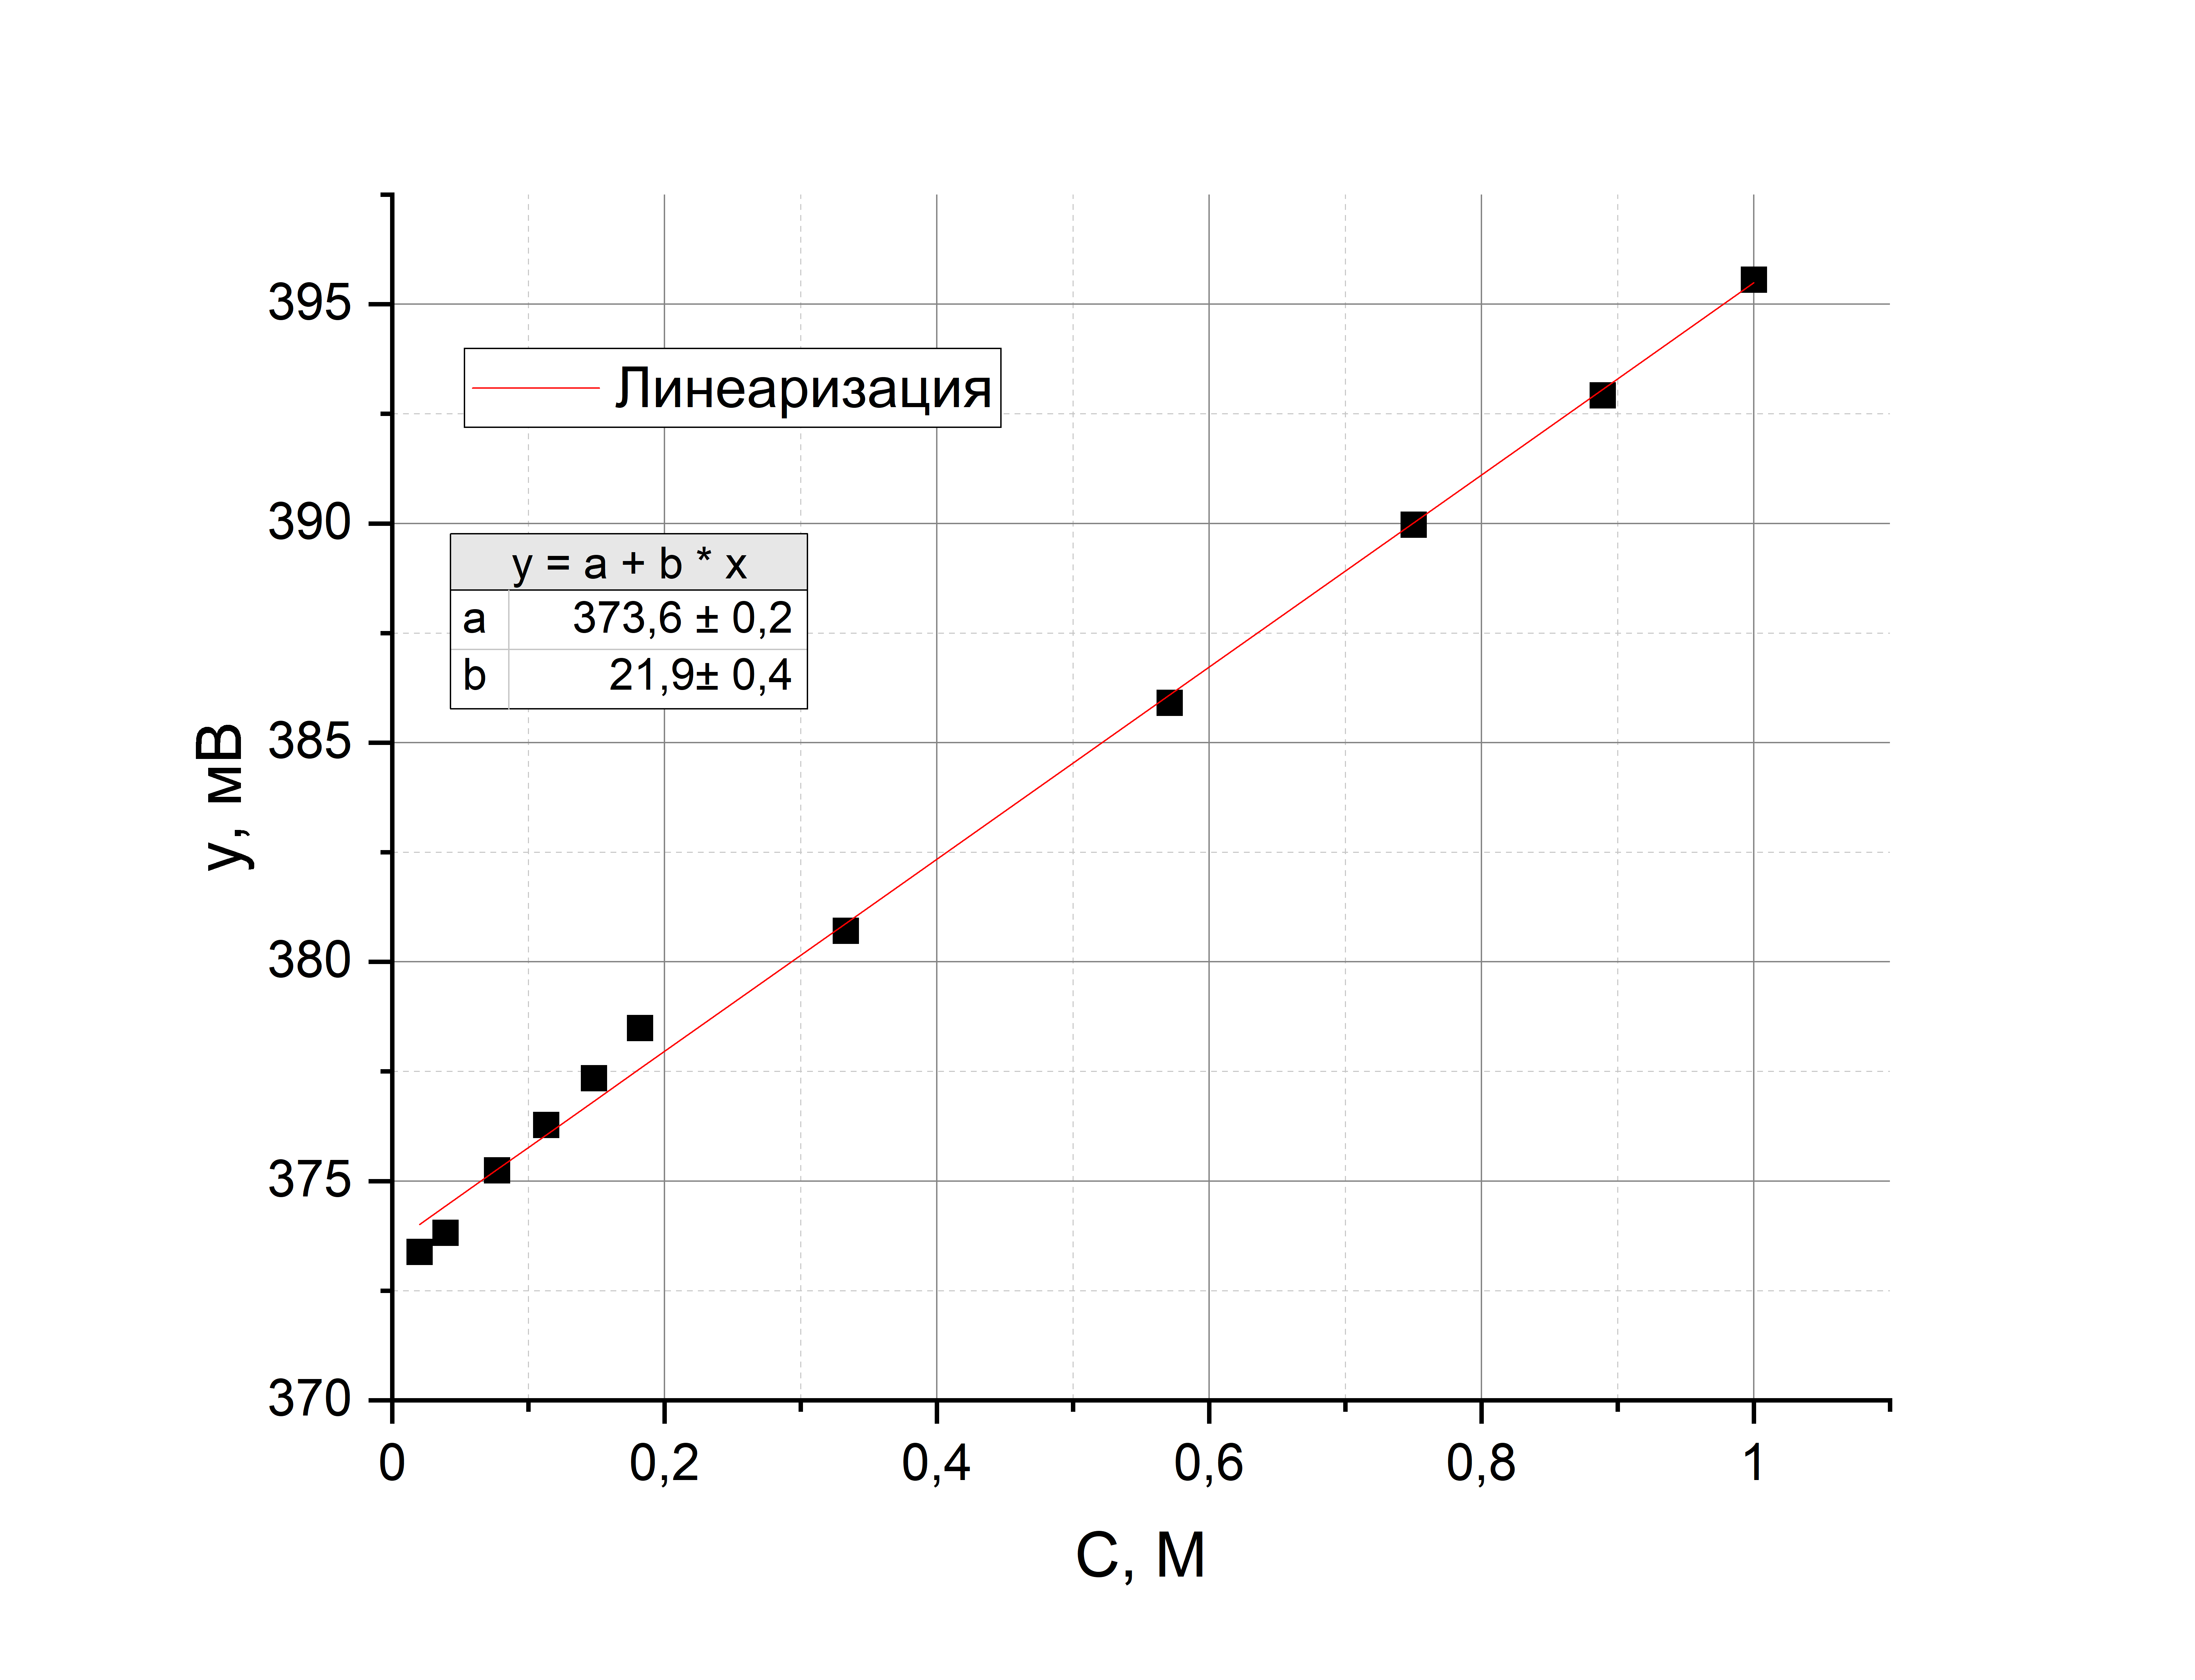
\includegraphics[width=0.7\textwidth]{3.3.png}
    \end{center}
    \caption{Зависимость $y(C_{HCl})$}
\end{figure}
\begin{figure}[h!]
    \begin{center}
    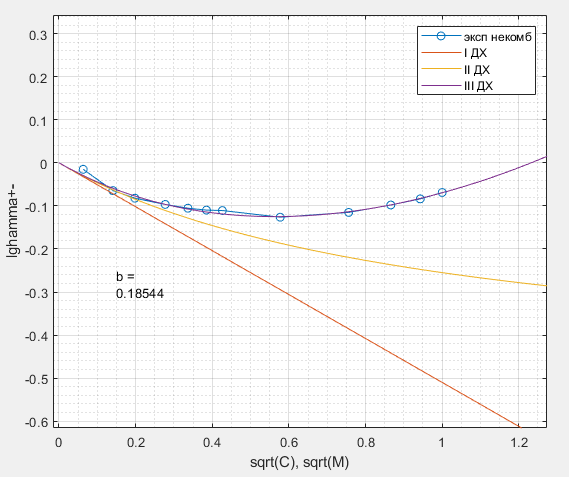
\includegraphics[width=0.7\textwidth]{3_5_I_II_III.png}
    \end{center}
    \caption{Зависимость $lg \gamma _{\pm}$ от $\sqrt{I}$}
\end{figure}

\subsubsection{Анализ серии измерений для комб. эл-да}
Зная калибровочные коэффициенты $a = 484 \pm 4$мВ и $b=-55.1 \pm 0.6$мВ из пункта 2.1, можно выразить логарифм коэффициента активности через показания комб. эл-да, как
\begin{equation}
    -pH=\frac{E_{X} - a}{b}= lg\gamma _{+} + lgC \mapsto lg\gamma _{+}=\frac{E_{X} - a}{b} - lgC
\end{equation}
Расчетные значения представлены в таблице 3, график на рисунке 5.
\begin{figure}[h!]
    \begin{center}
    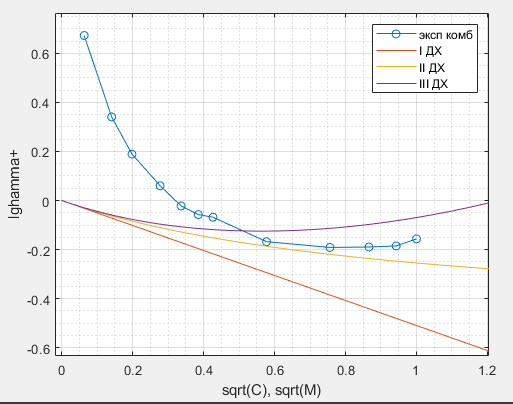
\includegraphics[width=0.7\textwidth]{3_6_lghamma_sqrtC_komb.png}
    \end{center}
    \caption{T(n)}
\end{figure}

\textbf{Вывод:} Стеклянный электрод лучше подходит для измерения коэффициента активности, так как в нем остутсвует жидкостное соединение, а значит и диффузионный потенциал, искажаюющий выдаваемое значение ЭДС. Как мы можем видеть на низких концентрациях рассчетный коэффициент активности для $H^{+}$ больше единицы, а если рассчитать с использованием калибровочных данных значение $pH$ раствора соляной кислоты концентрации 0.004М, получится 1.83 (что сильно ниже $pC = 2.4$). 

\subsection{Измерение проводимости раствора уксусной кислоты}
Соответсвующие измерения приведены в табл. 5. Из закона разбавления Оствальда следует, что для слабодиссоциирующей уксусной кислоты
\begin{equation}
    \alpha \cong \sqrt{\frac{K}{C}}
\end{equation}
Проводимость можно выразить как
\begin{equation}
    \kappa = nC\lambda_{\text{экв}} = [n = 1] = C\alpha \lambda_{\text{экв}}^{0} \cong \lambda^{0} \sqrt{KC}, \text{ где}
\end{equation}
$$\lambda^{0} = \lambda^{0}_{} + \lambda^{0}_{} = (349.8 + 40.9) \cdot 10^{-4} = 390.7 \cdot 10^{-4} \frac{\text{См}}{\text{м}^{2} \cdot \text{M}}$$ \footnote{Сухотин А. М., "Справочник по электрохимии"}
Таким образом, лианеризовав зависимость $\kappa$ от квдаратного корня из концентрации, можно рассчитать $K_{a}$ как
$$
K_{a} = (\frac{k_{\text{накл.}}}{\lambda^{0}})^{2} = (3.19 \pm 0.23) \cdot 10 ^{-5}, pK_{a} = 4.50 \pm 0.03 
$$
Справочные значения соответственно равны
$$ K_{a} = 1.75 \cdot 10 ^{-5}, pK_{a} = 4.75 \text{ } \footnote{Никольский Б.П., "Справочник химика"} $$
На рисунках 6 и 7 представлины графики зависимости $\kappa$ от $\sqrt{C}$ и $C$ соответсвенно. 
\begin{table}[h!]
\begin{center}
\caption{Зависимость удельной эл-пр-ти раствора от концентрации уксусной кислоты}
\begin{tabular}{|c|c|c|c|}
\hline
$\sqrt{C}, M^{-1}$ & $C$, Моль &$\kappa$, мкСм/см & \multicolumn{1}{l|}{\alpha} \\ \hline
0,032       & 0,001   & 74,8           & 0,191                  \\ \hline
0,134       & 0,018   & 329            & 0,047                  \\ \hline
0,270       & 0,073   & 670            & 0,023                  \\ \hline
0,405       & 0,164   & 1001           & 0,016                  \\ \hline
0,540       & 0,292   & 1235           & 0,011                  \\ \hline
0,707       & 0,5     & 1562           & 0,008                  \\ \hline
\end{tabular}
\end{center}
\end{table}


\begin{figure}[h!]
    \begin{center}
    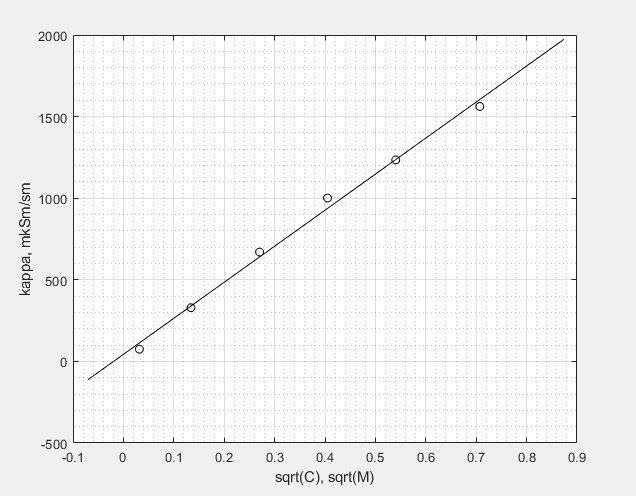
\includegraphics[width=0.7\textwidth]{4_1_kappa_sqrt.png}
    \end{center}
    \caption{$\kappa(\sqrt{C})$}
\end{figure}

\begin{figure}[h!]
    \begin{center}
    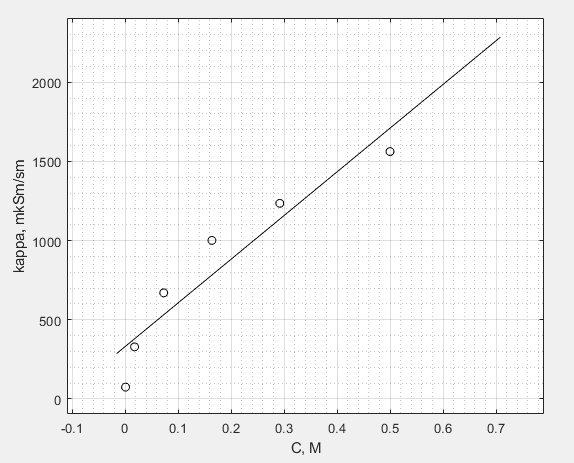
\includegraphics[width=0.7\textwidth]{4_2_kappa_C.png}
    \end{center}
    \caption{$\kappa(C)$}
\end{figure}

\newpage
%\subsection{Обработка результатов измерений}

 \section{Выводы}
\begin{enumerate}
    \item Потенциометрическим методом (с помощью некомбинированного электрода: референсный – хлорсеребряный, индикаторный - стеклянный) определен среднеионный коэфф активности НСl . Полученная зависимость $\gamma_{\pm}(\sqrt{C})$ соответствует третьему приближению теории Дебая-Хюккеля и второму приближению  при С < 0.05М. Оценить соответствие первому приближению (предельный закон Дебая-Хюккеля) не представляется возможным из-за того, что на малых С точность измерений ниже. 
    \item Кондуктометрическим методом определена зависимость удельной электропроводности р-ра уксусной кислоты от её концентрации (линейно по корню из С). С использованием закона разбавления Оствальда рассчитана константа диссоциации $К_{а}$ уксусной к-ты. Величина отличается от справочной в 1.7 раз.

\end{enumerate}

\end{document}
